\subsection{Model-Class Gauge Comparison}
\label{sec:model_class_comparison}

We compare one invariant class and three coordinate-dependent observers:
\[
\text{Invariant:}\quad
\frac{dm}{d\tau}=\beta-\lambda m,\quad
\Delta P = k\,[m(\tau_T)-m(\tau_0)].
\]
\[
\text{Coordinate surprise:}\quad
\frac{dm}{d\tau}=\beta I(\tau)-\lambda m,\quad
I(\tau)=\left|\frac{d\log(dt/d\tau)}{d\tau}\right|,\quad
\Delta P = k\,[m(\tau_T)-m(\tau_0)].
\]
\[
H_1(t)=|\dot\tau(t)-1|,\quad P_{H_1}=\int H_1(t)\,dt,\qquad
H_2(t)=|\ddot\tau(t)|,\quad P_{H_2}=\int H_2(t)\,dt.
\]

\paragraph{Warp metric and gate policy.}
For each model we compute
\[
\Delta P_{\text{warp}}=|P(\tau)-P(\tau\circ s)|.
\]
Family A ($\tau=t$) is sanity-only; Family B ($\tau=T(t/T)^{1.2}$) is the separation gate.
Ratios use the reported floor denominator from the same run:
\[
\mathrm{ratio}=\frac{\max\_error}{\max(\max\_error_{\text{inv}},\epsilon_{\text{floor}})}.
\]

\begin{figure}[H]
\centering
\begin{subfigure}[t]{0.49\linewidth}
  \centering
  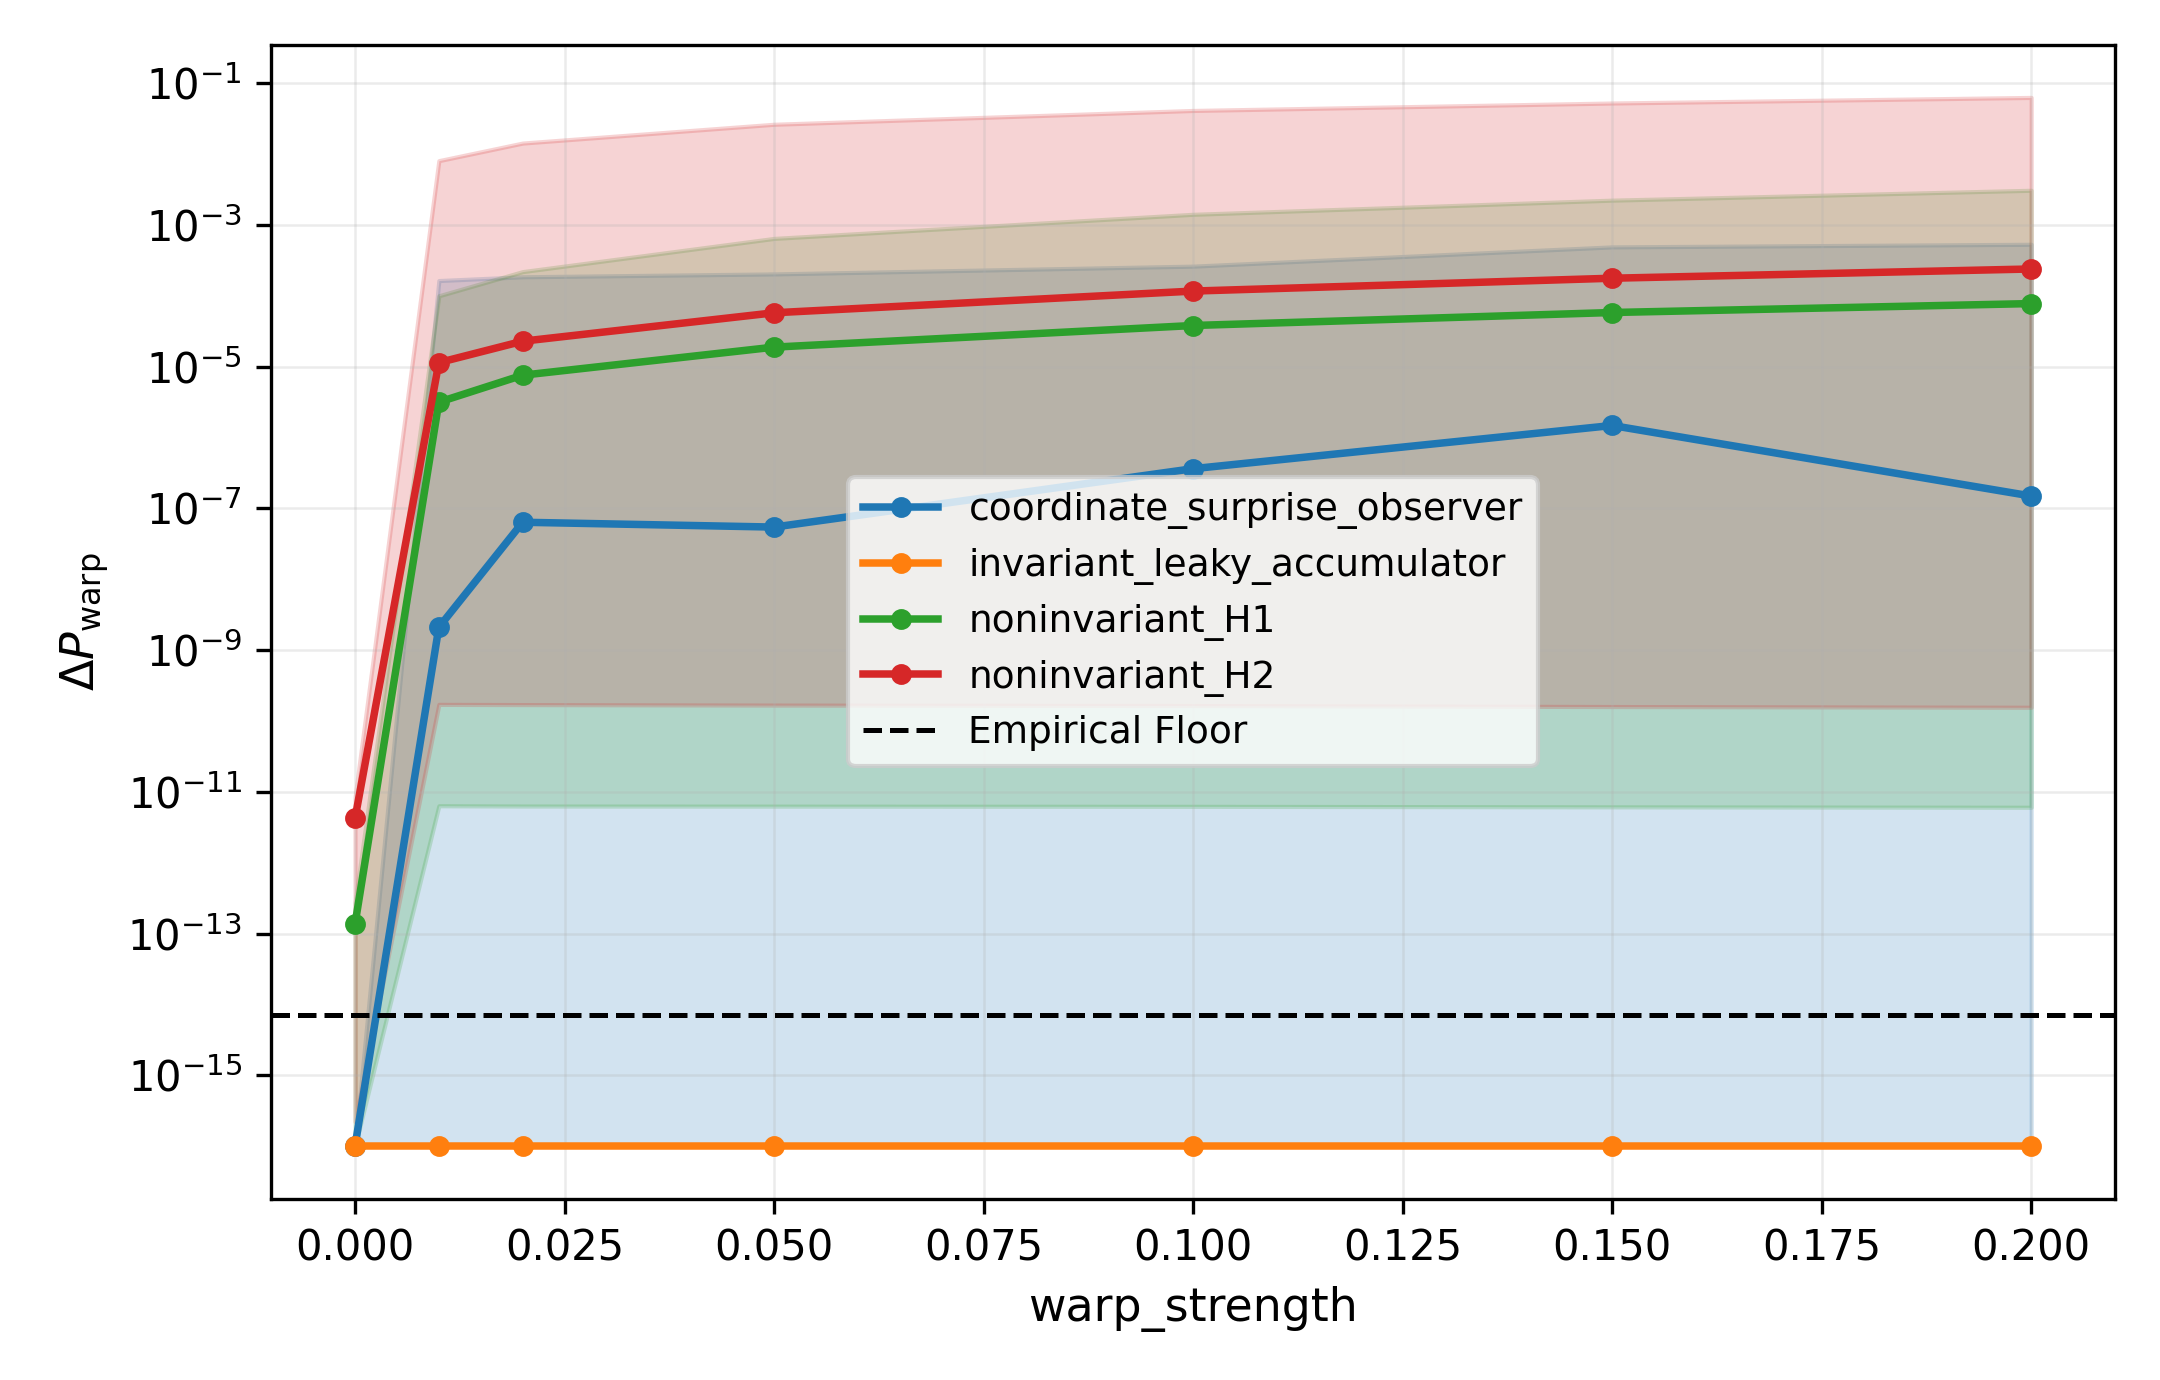
\includegraphics[width=\linewidth]{plots/main_fig1_warp_sweep.png}
  \caption{Warp-strength sweep using per-warp samples (median with p5--p95 band).}
\end{subfigure}
\hfill
\begin{subfigure}[t]{0.49\linewidth}
  \centering
  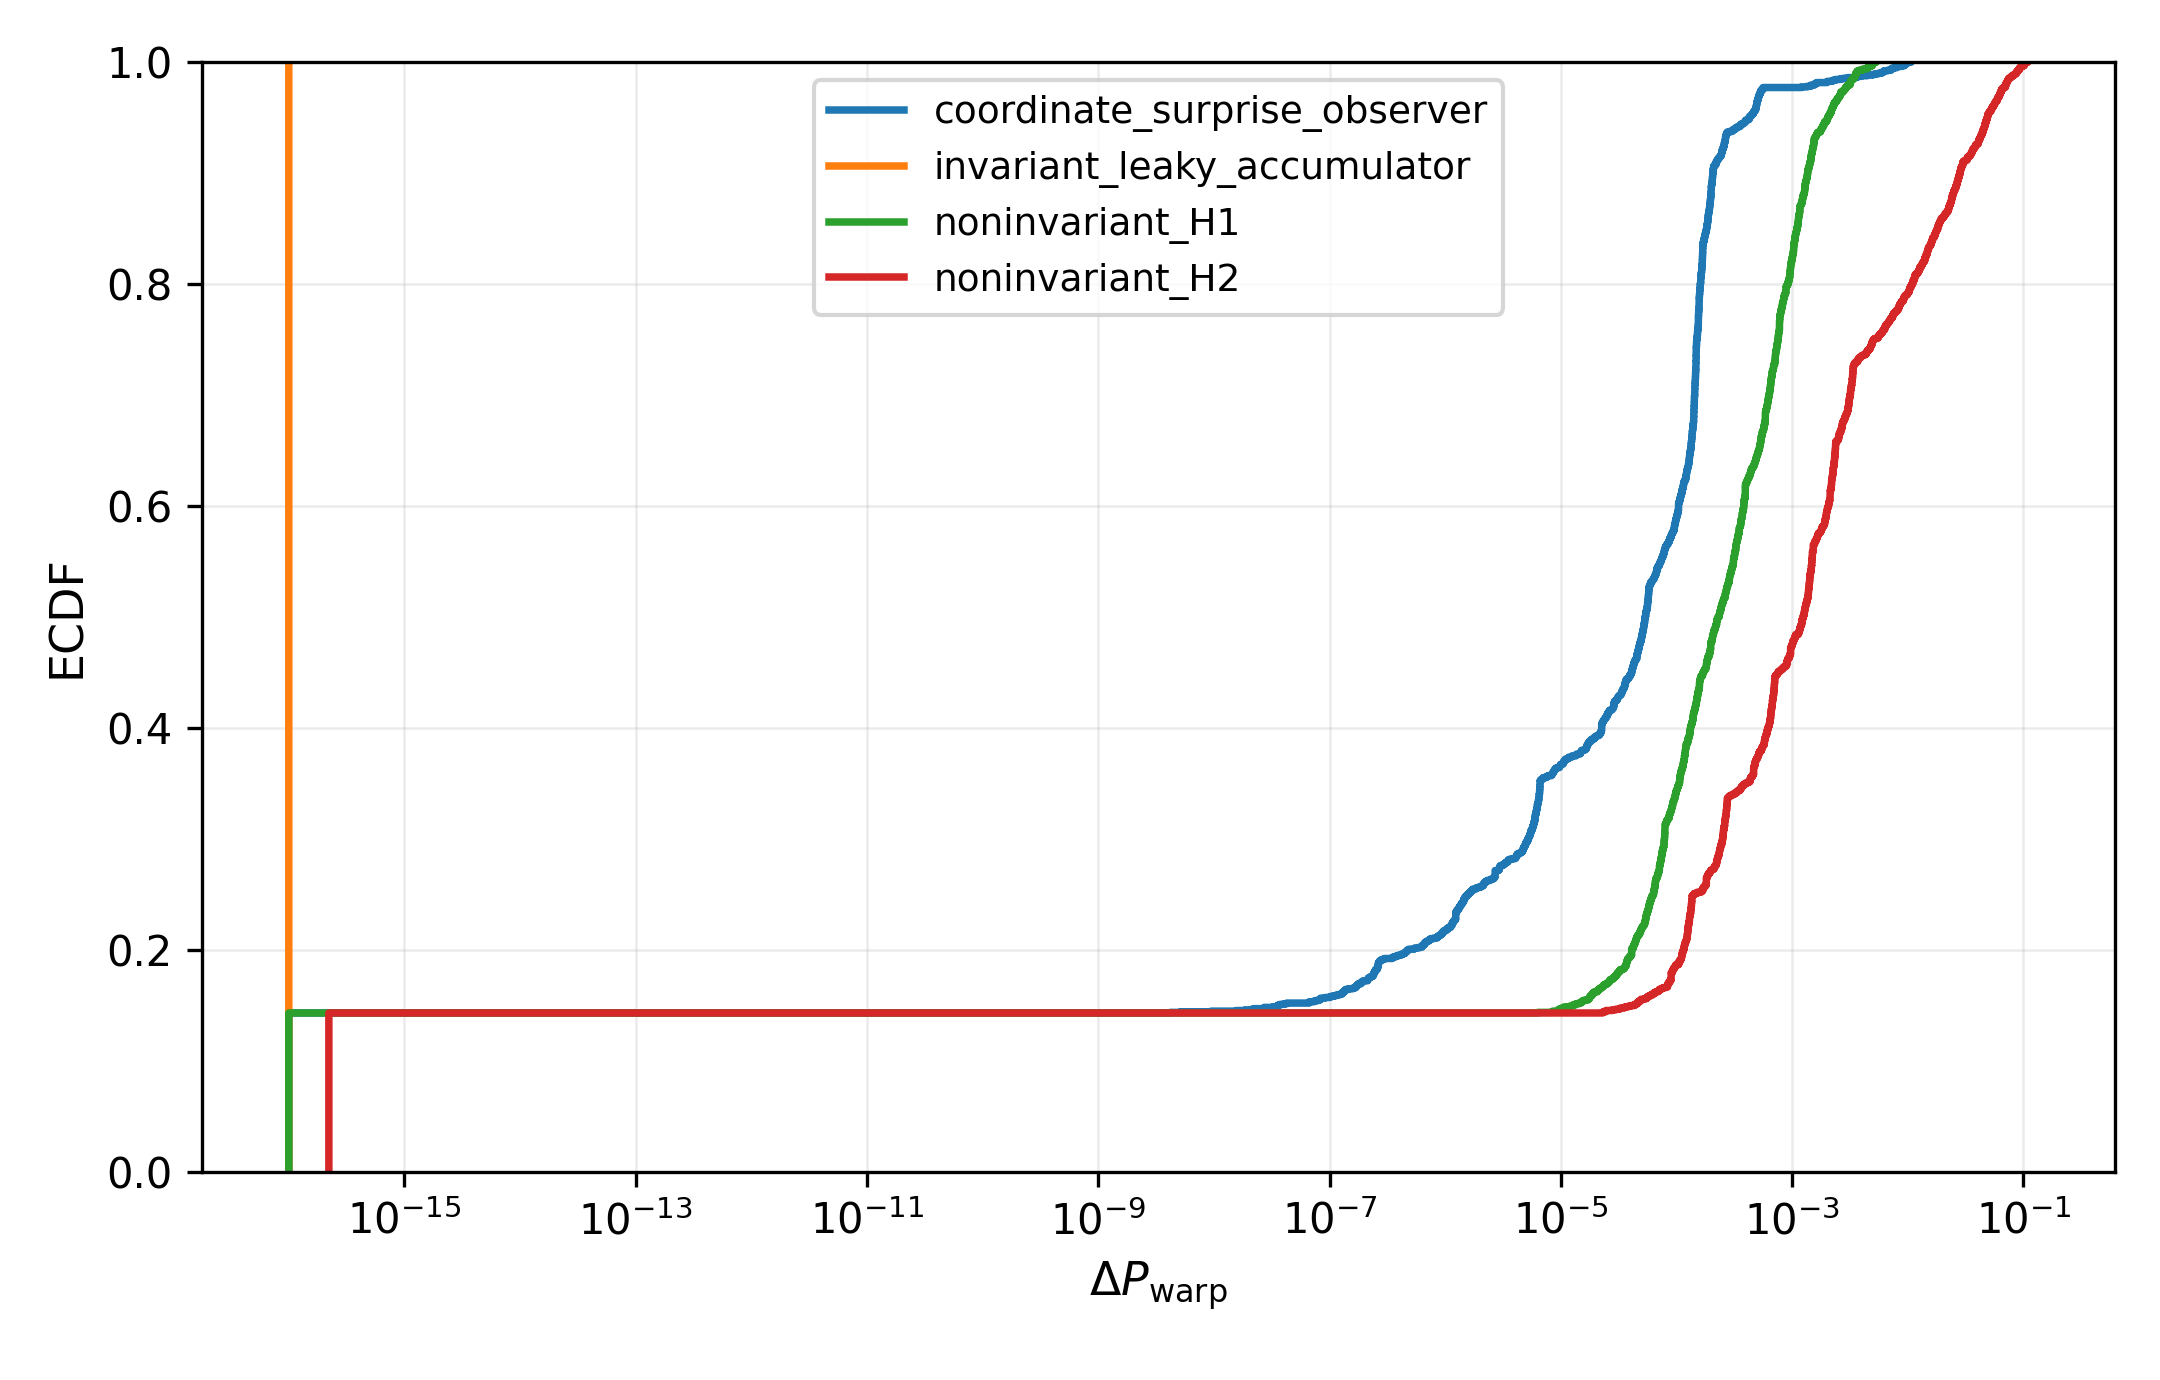
\includegraphics[width=\linewidth]{plots/main_fig2_ecdf_familyB.png}
  \caption{Family-B ECDF of $\Delta P_{\mathrm{warp}}$ by model class.}
\end{subfigure}
\caption{Main gauge-comparison figures generated from \texttt{per\_warp\_results.csv} and \texttt{gauge\_violation\_comparison.csv}.}
\label{fig:main_gauge_figures}
\end{figure}

\paragraph{Final separation (\texttt{paper\_final\_20260302}, Family B).}
Using \texttt{tables/gauge\_violation\_comparison.csv}:
\begin{table}[H]
\centering
\caption{Family-B gauge-violation separation using
\[
\mathrm{ratio\_to\_invariant}
=
\frac{\mathrm{max\_error}}{\epsilon_{\mathrm{floor,used}}},
\qquad
\epsilon_{\mathrm{floor,used}}=\max(\mathrm{EPS\_FLOOR},\epsilon_{\mathrm{floor,empirical}}).
\]
The invariant baseline is reported as $\mathrm{max\_error}=0$ (within floor) and ratio $=1.0$.}
\label{tab:gauge_violation_final_B}
\begin{tabular}{@{}lcc@{}}
\toprule
Model & max\_error & ratio\_to\_invariant \\
\midrule
Invariant leaky accumulator & 0 & 1.0 \\
Coordinate-surprise observer & $2.574388685956\times 10^{-2}$ & $3.660237056255\times 10^{12}$ \\
H1 & $3.619835733440\times 10^{-2}$ & $5.146641981986\times 10^{12}$ \\
H2 & $2.134064697311\times 10^{-1}$ & $3.034189331298\times 10^{13}$ \\
\bottomrule
\end{tabular}
\end{table}

All noninvariant observers pass the separation gate ($\ge 10^6$) by multiple orders of magnitude, while the invariant class remains at numerical floor.
